\chapter{Cardioline Specific ecosystem}
Cardioline is present on the market from the early 60s, they started developing and producing innovative machines to record the heart acivity. Nowadays their thecnology improved, making their products producing documents in a digital format.
Thus the company started to sell a system able to produce heart rate monitoring digital documents for different methodologies, forward them to a Software for the storage, alert the physicians and let them write their own examination.
\section{Software and Frameworks involved}
The managment software tool is based on the .NET platform, since the 32-bit libraries for the SCP-ECG format are microsoft technologies based.
Cardioline provides each customer with a Windows Server Machine running their webapplications realized with ASP .NET.
\section{Project target And System requirements}
The scope is to provide future customers with additional features of the managment application, avoiding the burden to keep up and running their own machines and infrastructure.
While Respecting the European jurisprudence in privacy subject, integrating their system with the national e-healthcare system.
Centralizing such services involved some problems,
\begin{itemize}
    \item High network and computing load
    \item New security policies for data
    \item Adoption of the international HL7 standard
    \item Continuity with legacy software
\end{itemize}
\section{Provider choice}
It has been decided to face the computing and network load problem using Computing Cloud technologies, since they let the developer choose the desired grade of control and customization over the system, and how to structure the network.
In particular the principal Cloud Computing providers offers this kinds of services
\begin{itemize}
    \item Saas
    \item Paas
    \item Iaas
\end{itemize}
And different kind of network topology such as
\begin{itemize}
    \item Private cloud
    \item Public cloud
\end{itemize}

\section{System Architecture}
As shown in the picture \ref{fig:architecture}, several Amazon Web Services were used to develop the Cardioline's Cloud infrastructure.
Everything but the SES Service is hosted in the eu-central-1 region in Frankfurt. Such region is divided into availability zones connected through low-latency links, in order to handle potential instance failures by replacing those failed instances with the standby ones placed in a different availability zone.\\

\begin{figure}[h]
    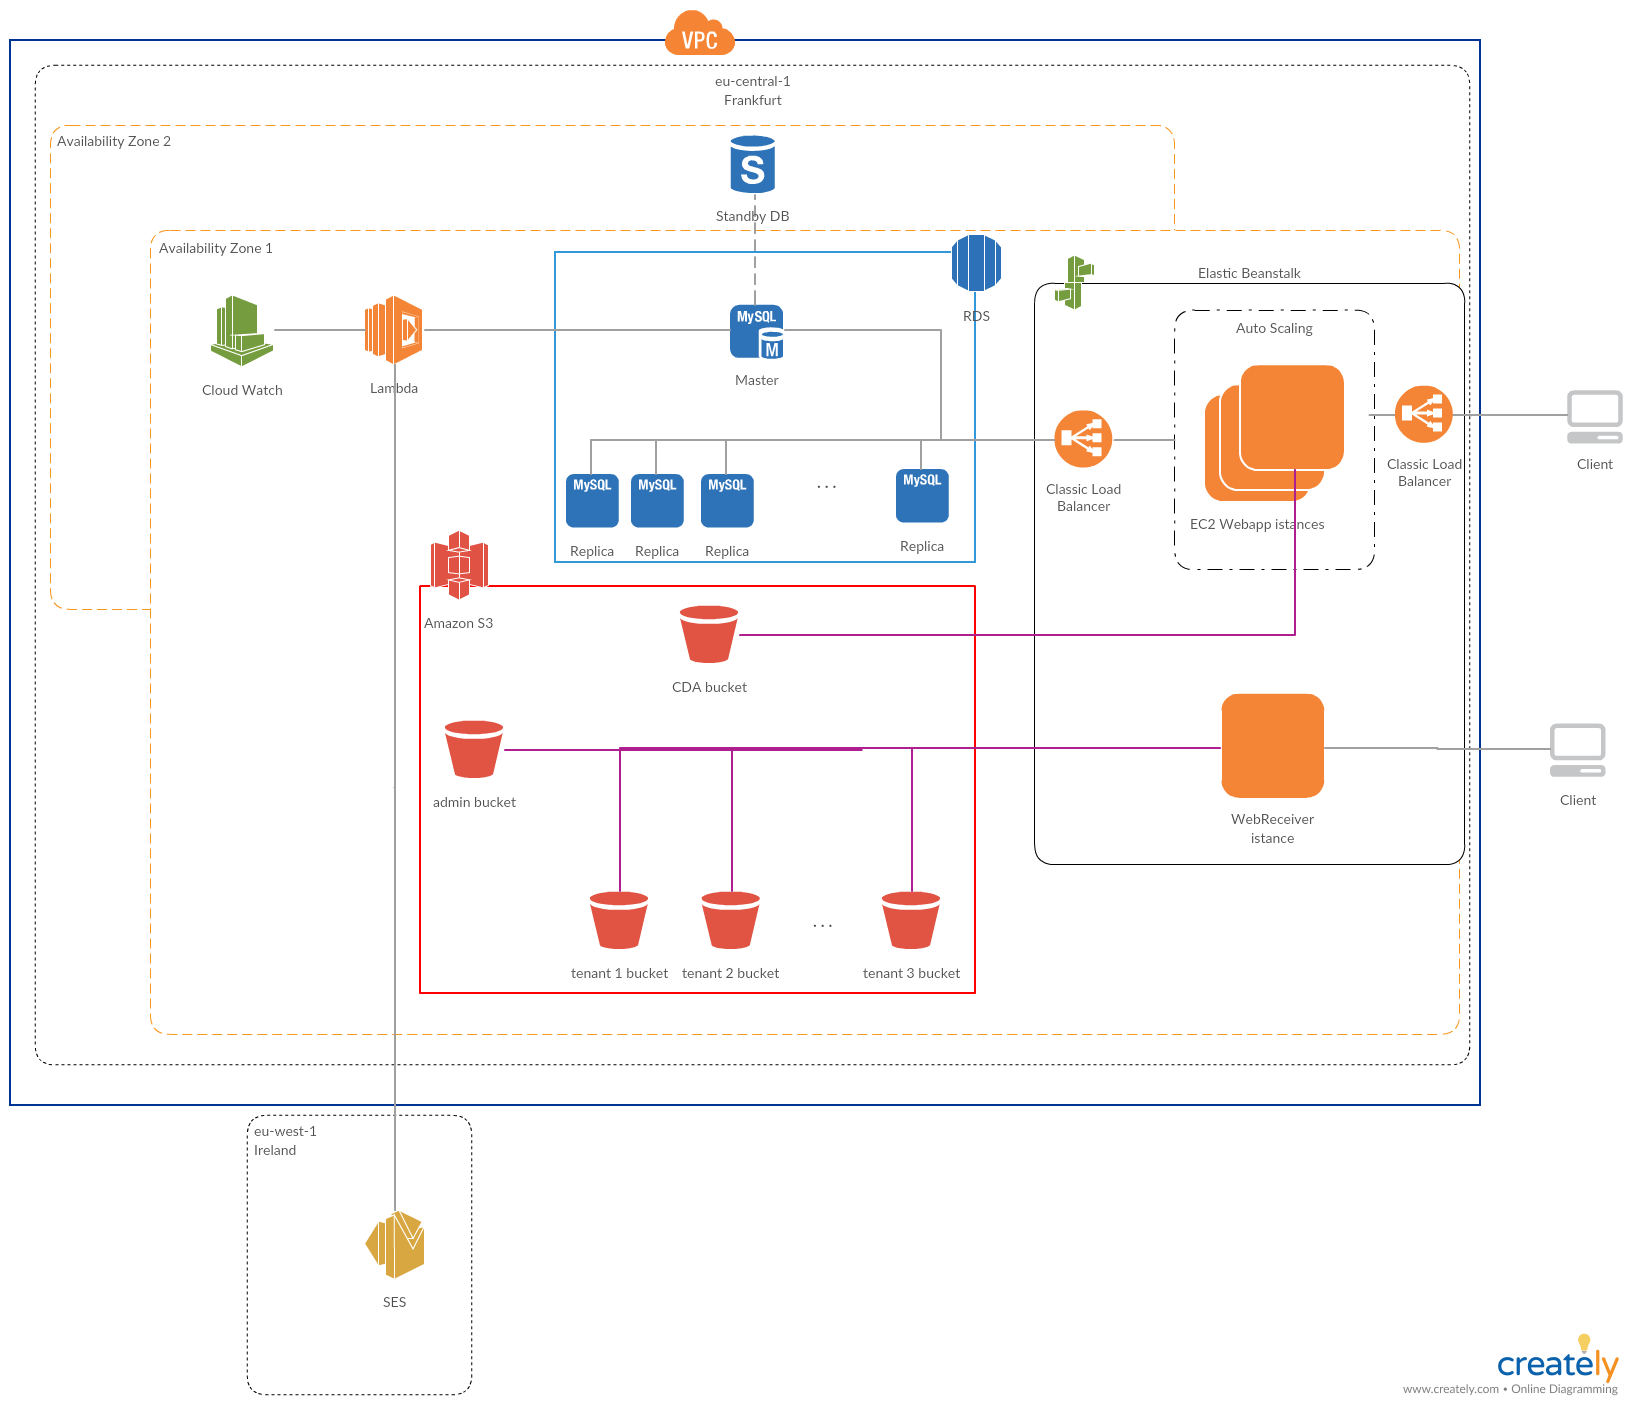
\includegraphics[width=\textwidth]{architecture}
    \caption{a nice plot}
    \label{fig:architecture}
\end{figure}